\documentclass[tikz,border=6mm]{standalone}
\usepackage{amsmath,amssymb}
\usepackage{fontspec}

\usetikzlibrary{positioning,arrows.meta,shapes.geometric,fit,backgrounds,calc}

% Master Academic Palette (WCAG AA & Color-Vision Deficiency Compliant)
\definecolor{navyblue}{RGB}{30, 60, 105}    % #1E3C69 - Model architectures, encoders, primary flows
\definecolor{tealblue}{RGB}{20, 110, 105}   % #146E69 - Data plane, ingestion, datasets, gold annotations
\definecolor{purplecat}{RGB}{95, 45, 120}   % #5F2D78 - Multi-task balancing, loss dynamics, statistics
\definecolor{ambergold}{RGB}{180, 85, 15}   % #B4550F - Hardware testbed, serving trials, embeddings
\definecolor{forestgreen}{RGB}{25, 115, 60} % #19733C - Acceptance gates, verified thresholds
\definecolor{crimsonred}{RGB}{175, 40, 40}  % #AF2828 - Feedback loops, out-of-domain holdouts, errors
\definecolor{slategrey}{RGB}{70, 85, 100}   % #465564 - Neutral boundaries, containers, baseline nodes

% Semantic aliases for use-case views
\colorlet{sysgray}{slategrey}
\colorlet{ucblue}{navyblue}
\colorlet{extpurple}{purplecat}
\definecolor{actorcolor}{RGB}{25, 35, 45}

% Actor stick figure pic
\tikzset{
    actorpic/.pic={
        % Head
        \draw[thick, draw=actorcolor, fill=actorcolor!10] (0,0.50) circle (0.20);
        % Body
        \draw[thick, draw=actorcolor] (0,0.30) -- (0,-0.20);
        % Arms
        \draw[thick, draw=actorcolor] (-0.38,0.10) -- (0.38,0.10);
        % Left Leg
        \draw[thick, draw=actorcolor] (0,-0.20) -- (-0.26,-0.60);
        % Right Leg
        \draw[thick, draw=actorcolor] (0,-0.20) -- (0.26,-0.60);
    },
    systemactorpic/.pic={
        % UML icon representing an automated software actor / external system
        \draw[thick, draw=actorcolor, fill=actorcolor!10, rounded corners=3pt] (-0.45,-0.30) rectangle (0.45,0.30);
        \node[font=\tiny\bfseries, text=actorcolor] at (0,0) {$\ll\text{service}\gg$};
    }
}

\begin{document}
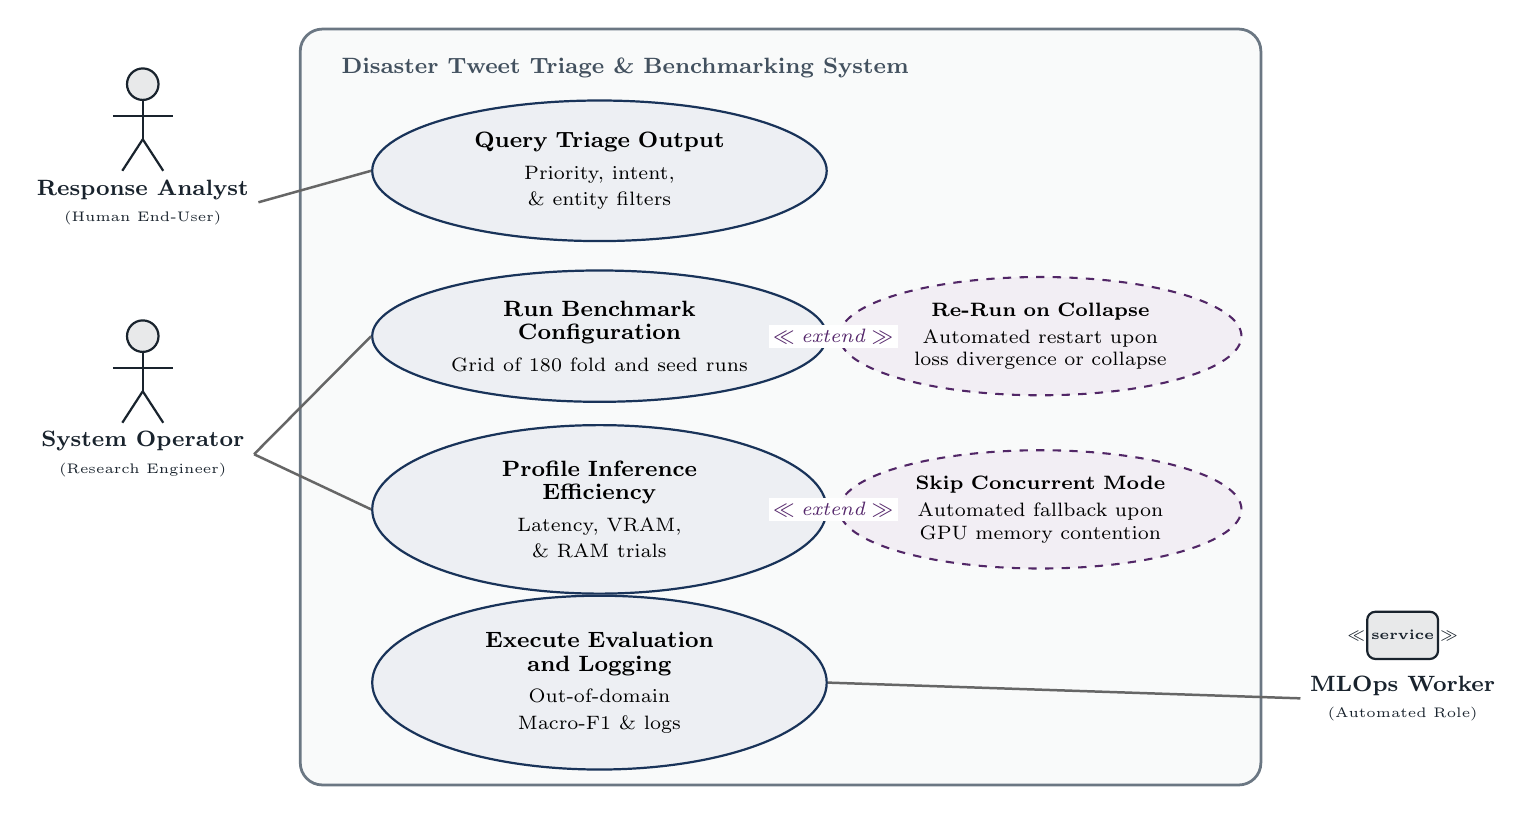
\begin{tikzpicture}[
    font=\small,
    >=Stealth,
    % Use case styles
    usecase/.style={
        draw=ucblue!85!black,
        fill=ucblue!8,
        ellipse,
        align=center,
        inner sep=4pt,
        font=\footnotesize,
        line width=0.8pt,
        text width=3.8cm,
        minimum height=1.25cm
    },
    extcase/.style={
        draw=extpurple!85!black,
        fill=extpurple!8,
        ellipse,
        dashed,
        align=center,
        inner sep=3pt,
        font=\scriptsize,
        line width=0.75pt,
        text width=3.4cm,
        minimum height=1.15cm
    },
    assoc/.style={
        draw=gray!80!black,
        line width=0.9pt
    },
    extendarrow/.style={
        ->,
        dashed,
        line width=0.8pt,
        draw=extpurple!85!black
    },
    stereolabel/.style={
        font=\scriptsize\itshape,
        text=extpurple!90!black,
        fill=white,
        inner sep=1.5pt
    },
    actornode/.style={
        align=center,
        font=\footnotesize\bfseries,
        text=actorcolor
    }
]

    % =========================================================================
    % 1. SYSTEM BOUNDARY BOX
    % =========================================================================
    \draw[draw=sysgray!80, fill=sysgray!3, rounded corners=8pt, line width=1.0pt]
        (0, -8.0) rectangle (12.2, 1.6);
    \node[anchor=north west, font=\bfseries\footnotesize, text=sysgray!95!black] 
        at (0.4, 1.35) {Disaster Tweet Triage \& Benchmarking System};

    % =========================================================================
    % 2. PRIMARY USE CASES (Inside Boundary)
    % =========================================================================
    % UC1: Query Triage Output (Top)
    \node[usecase] (uc1) at (3.8, -0.2) {
        \textbf{Query Triage Output}\\[2pt]
        \scriptsize Priority, intent, \& entity filters
    };

    % UC2: Run Benchmark Configuration (Upper Middle)
    \node[usecase] (uc2) at (3.8, -2.3) {
        \textbf{Run Benchmark}\\[-1pt]
        \textbf{Configuration}\\[2pt]
        \scriptsize Grid of 180 fold and seed runs
    };

    % UC4: Profile Inference Efficiency (Lower Middle)
    \node[usecase] (uc4) at (3.8, -4.5) {
        \textbf{Profile Inference}\\[-1pt]
        \textbf{Efficiency}\\[2pt]
        \scriptsize Latency, VRAM, \& RAM trials
    };

    % UC3: Execute Evaluation and Logging (Bottom)
    \node[usecase] (uc3) at (3.8, -6.7) {
        \textbf{Execute Evaluation}\\[-1pt]
        \textbf{and Logging}\\[2pt]
        \scriptsize Out-of-domain Macro-F1 \& logs
    };

    % =========================================================================
    % 3. EXTENSION USE CASES (Inside Boundary, Right Side)
    % =========================================================================
    % Extension to UC2: Re-run on Loss Collapse
    \node[extcase] (ext_collapse) at (9.4, -2.3) {
        \textbf{Re-Run on Collapse}\\[2pt]
        \scriptsize Automated restart upon loss divergence or collapse
    };

    % Extension to UC4: Skip Concurrent on Memory Contention
    \node[extcase] (ext_contention) at (9.4, -4.5) {
        \textbf{Skip Concurrent Mode}\\[2pt]
        \scriptsize Automated fallback upon GPU memory contention
    };

    % Extend Relationships (Dashed arrows from Extension to Base Use Case)
    \draw[extendarrow] (ext_collapse) -- (uc2) 
        node[midway, stereolabel] {$\ll\text{extend}\gg$};

    \draw[extendarrow] (ext_contention) -- (uc4) 
        node[midway, stereolabel] {$\ll\text{extend}\gg$};

    % =========================================================================
    % 4. ACTORS (Outside Boundary)
    % =========================================================================

    % Left Human Actor 1: Response Analyst (Associated with UC1)
    \pic at (-2.0, 0.4) {actorpic};
    \node[actornode] (actor_analyst) at (-2.0, -0.6) {
        Response Analyst\\
        \tiny\normalfont (Human End-User)
    };

    % Left Human Actor 2: System Operator (Associated with UC2 and UC4)
    \pic at (-2.0, -2.8) {actorpic};
    \node[actornode] (actor_operator) at (-2.0, -3.8) {
        System Operator\\
        \tiny\normalfont (Research Engineer)
    };

    % Right Automated Actor: MLOps Worker (Associated with UC3)
    \pic at (14.0, -6.1) {systemactorpic};
    \node[actornode] (actor_mlops) at (14.0, -6.9) {
        MLOps Worker\\
        \tiny\normalfont (Automated Role)
    };

    % =========================================================================
    % 5. ASSOCIATIONS (Solid lines connecting Actors to Use Cases)
    % =========================================================================
    % Analyst to UC1
    \draw[assoc] (actor_analyst.east) -- (uc1.west);

    % Operator to UC2 and UC4
    \draw[assoc] (actor_operator.east) -- (uc2.west);
    \draw[assoc] (actor_operator.east) -- (uc4.west);

    % MLOps Worker to UC3
    \draw[assoc] (actor_mlops.west) -- (uc3.east);

\end{tikzpicture}
\end{document}
